\documentclass[11pt,letterpaper,boxed]{pset}

\usepackage[margin=0.75in]{geometry}
\usepackage{ulem}

\name{Name: \rule{2.5cm}{0.15mm}}
\assignment{Box \# \rule{1.5cm}{0.15mm}}
\class{MATH060 HW9}

\begin{document}

    \problemlist{MATH060 HW9}
    \begin{center}
    	5.4: 4, 5, 18, 29ab \\
    	5.5: 25, 31, 34, 38
    \end{center}
    
    \begin{problem} [5.4.4]
    	Find the value of $\iiint_W z \textrm{ } dV$, where $W=[-1,2] \times [2,5] \times [-3,3]$, without resorting to explicit calculation.
    \end{problem}
    \newpage
    
    
    \begin{problem} [5.4.5]
    	Evaluate the iterated integral.
    
    	\[\int_{-1}^2 \int_1^{z^2} \int_0^{y+z} 3yz^2 \textrm{ }dx\textrm{ }dy\textrm{ }dz\]
    
    \end{problem}
    \newpage
    
    
    \begin{problem} [5.4.18]
    	Integrate the given function over the indicated region $W$.
    
    	\[f(x,y,z)=z\]
    
    	$W$ is the region bounded by $z = 0, x^2 + 4y^2 = 4$, and $z = x + 2$. 
    \end{problem}
    \newpage
    
    
    \begin{problem} [5.4.29]
    	Consider the iterated integral
    
    	\[\int_{-2}^2 \int_0^{\frac12 \sqrt{4-x^2}} \int_{x^2+3y^2}^{4-y^2} 
    		(x^3+y^3) dz \textrm{ } dy \textrm{ } dx.\]
    
        \begin{enumerate}
            \item This integral is equal to a triple integral over a solid region $W$ in $\mathbb{R}^3$.
    		Describe $W$.
    		\item Set up an equivalent iterated integral by integrating first with respect to $z$, 
    		then with respect to $x$, then with respect to $y$. Do not evaluate your answer.
        \end{enumerate}
    \end{problem}
    \newpage
    
    \begin{problem} [5.5.25]
    	Evaluate 
    
    	\[\iint_D \textrm{cos} (x^2 + y^2)dA\]
    
    	where $D$ is the shaded region below.
    \end{problem}
    
    \begin{figure}[h!]
    	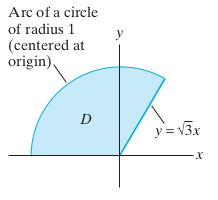
\includegraphics[width=60mm]{region.png}
    \end{figure}
    \newpage
    
    
    \begin{problem} [5.5.31]
    	Determine
    
    	\[\iiint_W (x^2+y^2+2z^2)\textrm{ }dV\]
    
    	where $W$ is the solid cylinder defined by the inequalities $x^2+y^2 \leq 4, -1 \leq z \leq 2.$
    \end{problem}
    \newpage
    
    
    \begin{problem} [5.5.34]
    	Determine the value of the given integral, where $W$ is the region bounded by the two spheres $x^2+y^2+z^2=a^2$ and $x^2+y^2+z^2=b^2$, for $0 < a < b$.
    
    	\[\iiint_W \frac{dV}{\sqrt{x^2+y^2+z^2}}\]
    \end{problem}
    \newpage
    
    
    \begin{problem} [5.5.38]
    	Determine
    
    	\[\iiint_W (2 + \sqrt{x^2+y^2})\textrm{ }dV\]
    
    	where $W = \{(x,y,z) : \sqrt{x^2+y^2} \leq z/2 \leq 3\}.$
    \end{problem}
    \newpage
    
\end{document}